\documentclass[11pt]{report}

% Packages
\usepackage{graphicx} % Required for inserting images
\usepackage{fancyhdr} % Headers & Footers
\usepackage{geometry} % Page Size and Margins
\usepackage{hyperref} % Make Hyper References (Links)
\usepackage{lastpage}
\usepackage{afterpage}
\usepackage{changepage}
\usepackage{soul}
\usepackage{todonotes}
\usepackage{makecell}
\usepackage{tabularx}

\usepackage{notoccite}
\usepackage{wrapfig}

\usepackage{csquotes}

%Changes the way the paragraph command behaves, now acts as a subsubsubsection
\makeatletter
\renewcommand\paragraph{\@startsection{paragraph}{4}{\z@}%
            {-2.5ex\@plus -1ex \@minus -.25ex}%
            {1.25ex \@plus .25ex}%
            {\normalfont\normalsize\bfseries}}
\makeatother
\setcounter{secnumdepth}{4} % how many sectioning levels to assign numbers to
\setcounter{tocdepth}{4}    % how many sectioning levels to show in ToC

\newcommand{\mychapter}[2]{
    \setcounter{chapter}{#1}
    \setcounter{section}{0}
    \chapter*{#2}
    \addcontentsline{toc}{chapter}{#2}
}

\pagestyle{fancy} 
\cfoot{\hfill \thepage/\pageref{LastPage}}
\rhead{Yohan's seq-toolbox}
\lhead{
\includegraphics[height=1cm]{CRESCO_1.png}{}}


%Changes the way the paragraph command behaves, now acts as a subsubsubsection
\makeatletter
\renewcommand\paragraph{\@startsection{paragraph}{4}{\z@}%
            {-2.5ex\@plus -1ex \@minus -.25ex}%
            {1.25ex \@plus .25ex}%
            {\normalfont\normalsize\bfseries}}
\makeatother
\setcounter{secnumdepth}{4} % how many sectioning levels to assign numbers to
\setcounter{tocdepth}{4}    % how many sectioning levels to show in ToC


\newcommand\blankpage{%
    \null
    \thispagestyle{empty}%
    \addtocounter{page}{-1}%
    \newpage}

\newcommand{\nocontentsline}[3]{}
\newcommand{\tocless}[2]{\bgroup\let\addcontentsline=\nocontentsline#1{#2}\egroup}

% for formal definitions
\usepackage{framed}
\usepackage{xcolor}
% environment derived from framed.sty: see leftbar environment definition
\definecolor{formalshade}{rgb}{0.95,0.95,1}
\definecolor{DarkPowderBlue}{rgb}{0.00,0.19,0.56}
\newenvironment{formal}{%
  \def\FrameCommand{%
    \hspace{1pt}%
    {\color{DarkPowderBlue}\vrule width 2pt}%
    {\color{formalshade}\vrule width 4pt}%
    \colorbox{formalshade}%
  }%
  \MakeFramed{\advance\hsize-\width\FrameRestore}%
  \noindent\hspace{-4.55pt}% disable indenting first paragraph
  \begin{adjustwidth}{}{7pt}%
  \vspace{2pt}\vspace{2pt}%
}
{%
  \vspace{2pt}\end{adjustwidth}\endMakeFramed%
}


%Different highlight colors
\definecolor{amber}{rgb}{1.0, 0.49, 0.0}
\definecolor{airforceblue}{rgb}{0.36, 0.54, 0.66}

\definecolor{custom_green}{RGB}{102,194,165}
\definecolor{custom_blue}{RGB}{141,160,203}

\DeclareRobustCommand{\hlorange}[1]{{\sethlcolor{amber}\hl{#1}}}
\DeclareRobustCommand{\hlsteelblue}[1]{{\sethlcolor{airforceblue}\hl{#1}}}

\DeclareRobustCommand{\hlgreen}[1]{{\sethlcolor{custom_green}\hl{#1}}}
\DeclareRobustCommand{\hlblue}[1]{{\sethlcolor{custom_blue}\hl{#1}}}

%\DeclareRobustCommand{\hlsteelblue}[1]{{\sethlcolor{airforceblue}\hl{#1}}}
%\DeclareRobustCommand{\hlsteelblue}[1]{{\sethlcolor{airforceblue}\hl{#1}}}



%Bash scripting
\usepackage{listings}
\lstdefinelanguage{bash}{
  keywords={if, then, else, elif, fi, for, while, do, done, until, case, esac, function, select, in},
  keywordstyle=\color{blue}\bfseries,
  ndkeywords={echo, printf, read, cd, ls, pwd, mkdir, rmdir, touch, cp, mv, rm, chmod, chown, grep, awk, sed, find, sudo, kill, ps},
  ndkeywordstyle=\color{purple}\bfseries,
  identifierstyle=\color{black},
  comment=[l]{\#},
  commentstyle=\color{gray}\itshape,
  stringstyle=\color{green},
  sensitive=true
}

\lstset{
  language=bash,
  frame=single,
  basicstyle=\ttfamily\small,
  backgroundcolor=\color{lightgray!20},
  showspaces=false,
  showstringspaces=false,
  showtabs=false,
  tabsize=2,
  breaklines=true,
  breakatwhitespace=true,
  numbers=left,
  numberstyle=\tiny,
  numbersep=5pt,
}


\title{From code to biology \\ A detailed (and simple) guide to the seq-toolbox}
\author{Yohan Lefol}
\date{\today}

\begin{document}
\maketitle

\section*{Purpose of this guide}
%\addtocounter{section}{1}
\thispagestyle{empty}
This report serves as a means to aid and guide individuals in the use of the seq-toolbox. The general idea is that this guide allows you to use the elements of the seq-toolbox, and if one desires it also offers sections/chapters on the details of the specific elements of the toolbox. This may be beneficial for the interpretation of some results as well as general knowledge of these bioinformatic tools.\\
This guide is intended to cover the various elements for different sequencing types, such as CHIPseq, sBliss (DSB break seq), and others... For now it only covers sBliss.\todo{May have to rework the section/subsection organization}\\

\section*{Notes to self - will remove eventually}
\begin{itemize}
\item Some of these sequencing methods can adjust what they measure (for example, DSBs, Okazaki fragments etc...) so plots will have to adjust for this. Or rather the analysis wrappers will need to know. It shall depend on the process of analysis I guess.
\item There are some commonalities between several pipelines. I may want to make them all the same in order to simply have one section for things like prepare and launch scripts. Currently CHIP and RNA are the same, sBLISS could be easily adapted. Since Chip is the same as ATAC that one also falls into the lump of `same'.
\end{itemize}
\clearpage

%Table of contents
{\small\tableofcontents}
\thispagestyle{empty}

\clearpage
\thispagestyle{empty}
\clearpage

\fancyhead[RO]{Installation}
\mychapter{1}{Installation} 
\label{chap:Install}
The installation utilizes several elements as unfortunately not both the tools used in the data processing and the tools used in the analysis cannot be reliably contained within a single environment. We divide this in two types of environment, a conda environment and a R environment. The conda environment covers the data processing side of the seq-toolbox while the R environment covers the data analysis side of things.

\section{Conda environments \label{sec:conda}}
In programming an environment is a self-contained isolated space where we can install specific versions of specific tools/packages. Having these tools stored in an environment means that one can easily provide a working environment to someone else, and that someone else will have the same tools and versions as was initially added into the environment.\\
Conda itself is a tool for managing environments. It was initially designed for Python however it has now been extended to R. This toolbox utilizes conda to manage python based data processing tools such as FastQC and Bowtie.\\
For more information, one can browse the conda website: \url{https://docs.conda.io/projects/conda/en/stable/}.\\
\section{Activating an environment}
Conda allows you to create multiple environments. In the case of this toolbox we have created one environment called `seq-toolbox'. To use this environment it must first be activated, this is accomplished by using a particular command in the terminal \autoref{sec:terminal}, as seen below:\\
\begin{lstlisting}
conda activate seq-toolbox
\end{lstlisting}
Once you have done this, the terminal should show that you have entered the inputted environment name.

\fancyhead[RO]{sBLISS}
\mychapter{2}{sBLISS}
\label{chap:BLISS_sBLISS}
Breaks Labeling In Situ and Sequencing or `BLISS' was introduced in 2017 \cite{yan2017bliss} and has since been re-made into in-Suspension Breaks Labeling In Situ and Sequencing or `sBLISS' \cite{bouwman2020genome}. sBLISS serves as a method to identify double-stranded breaks (DSBs) in a genome. From a bioinformatic perspective, this technology leverages Unique Molecular Identifiers (UMIs) to identify unique double stranded breaks as well as their location in the genome. See \autoref{fig:sbliss_workflow} for an overview of the protocol from a lab perspective.

\section{Scan for Matches \label{sec:scan_for_matches}}
The sBLISS pipeline utilizes scan\_for\_matches as an element of it's method, however the installation of this has become quite difficult. In order to install it on our local computer we had to use an old version of linux, do the installation, then export the file from /usr/bin/. This file was then transferred to the computer with a current linux version and manually inserted into it's /usr/bin/. This is not an ideal solution as it is quite difficult to replicate, if at all.\\
I have created a bash based script to substitute the scan\_for\_matches component used in the standard sBLISS pipeline. The sBLISS pipeline shipped with this toolbox comes equipped with this new method, however the old method remains in the main script, it is simply commented out.

\section{Adaptor anatomy \label{sec:sBliss_adaptors}}
\begin{itemize}
\item \textbf{T7 promoter sequence} - used for amplification
\item \textbf{RA5 adaptor} - Necessary for sequencing
\item \textbf{UMI} - Allows us to remove duplicates while processing the sequenced data
\item \textbf{Sample Barcode} - Used for demultiplexing (if required) and to quality control the data processing
\end{itemize}
Without going into details (yet) the T7 and RA5 elements are of no use in data processing, in which case they will have to be `trimmed' from the sequencing (fastq) files. It is likely that these have already been removed \todo{explain how to check this}.\\
The UMI and sample barcode are relevant, and recurring in the bioinformatic analysis. It is very important to know the length of each of these adaptors. Looking at the box below you can see a simplified example of a fastq file line. We have the header which provides a name and an contain some information between the colons (not always). For now this information is not relevant. The importance is to note the highlighted areas of the sequence. In this example the sample SRR11119500 has a UMI of AAAGGNAA and a sample barcode of CATCACGC. The UMI will be unique for each line of the fastq file while the sample barcode will always be the same. Knowing the sample barcode is essential for the proper functioning of the sBLISS pipeline as the program must know the barcode associated to each sample. By knowing the length and format of the adaptor we are capable of finding the sample barcode if it is no explicitly provided. In this experiment we knew that the UMI preceded the barcode and the UMI was of 8 nucleotides long, with the sample barcode having the same length. From this we could establish what the sample barcode was by taking nucleotides 8-16 of each line of the fastq file and checking which was the most recurring pattern. We have to check the entire file as there may be mismatches. This will be covered in more details later, however know that the pipeline will allow for no more than 1 mismatched nucleotide in a sample barcode.

\begin{formal}
@SRR11119500.1:::1:::length=76\\
\hlorange{AAAGGNAA}\hlsteelblue{CATCACGC}AGTGGTATTATAAGAAC[...]
\end{formal}

\begin{figure}
\centering
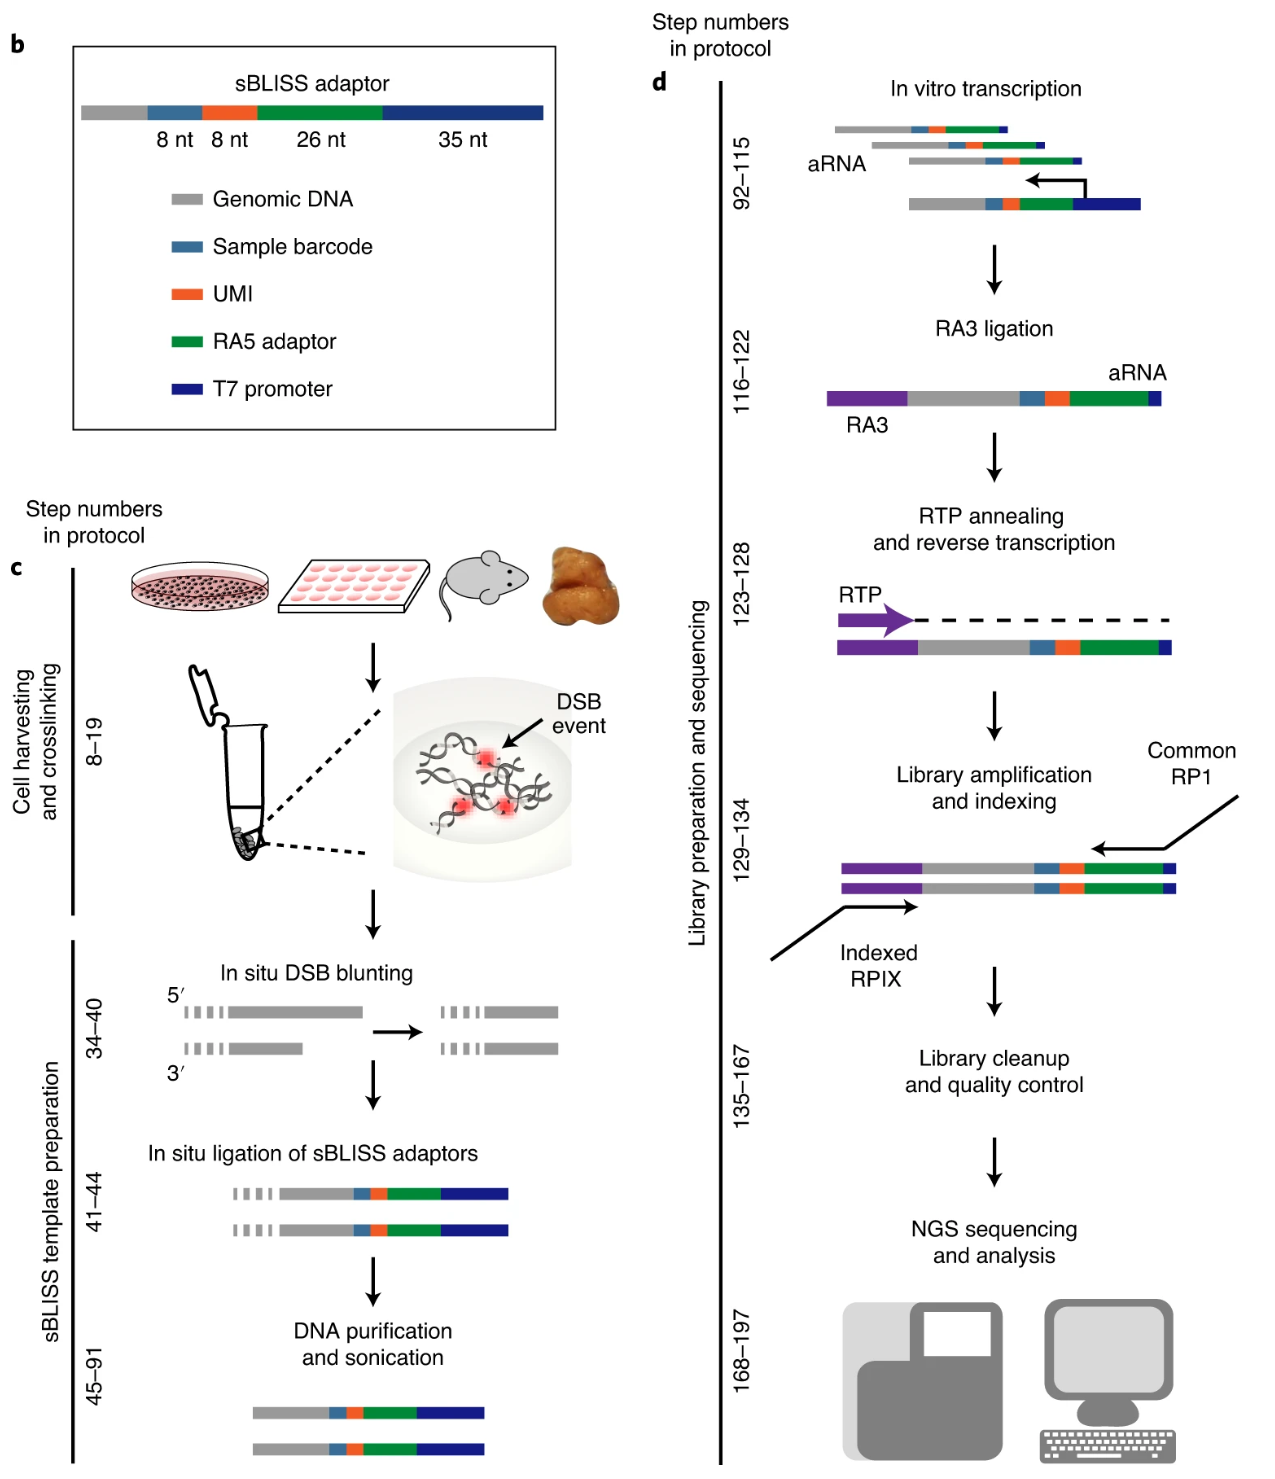
\includegraphics[width=12cm, height=14cm]{figures/sBLISS_workflow.png}
\caption{b, Sequence structure of the sBLISS adaptor. c and d, Step-by-step scheme of the protocol.\\
Figure from \protect\cite{bouwman2020genome} - figure 1}
\label{fig:sbliss_workflow}
\end{figure}

\section{Verify Fastq files \label{sec:sbliss_check_fastq}}
Fastq files can come in a variety of formats \autoref{sec:Fastq_files}, the sBLISS pipeline requires a relatively specific format. This is discussed in a github issue (\url{https://github.com/BiCroLab/blissNP/issues/6}). Essentially, some fastq files, especially those downloaded form NCBI or other repositories, may be incorrectly formatted for this pipeline. To check this, you can simply open the fastq file (you may have to extract it first). Open the fastq file using the `glogg' software \autoref{sec:glogg}. If you observe a format where the header (see the box in \autoref{sec:sBliss_adaptors} above) contains colons, then the format is likely to be correct. In the case where it contains no colons or fails a check (detailed below), you can run the `fix\_fastq\_format.sh' script with the following method:\\
\begin{enumerate}
\item Move to directory with the script
\begin{lstlisting}
cd seq_toolbox/sbliss/
\end{lstlisting}
\item Launch the script while providing a path to the directory
\begin{lstlisting}
bash fix_fastq_format.sh path_to_data
\end{lstlisting}
\end{enumerate}
Once the script is complete the directory you gave will contain files with the term 'fixed' appended to them. You should move these files to an alternate folder/location.\\
Additionally there is a check implemented on the script where an incorrect file format will usually result in a blank file. This is not a fool proof check though it does serve as an indication of a possible issue in the file format. The error will read
\begin{displayquote}
Error: r2.2b.aln.fq is empty. This may be due to incorrect fastq file format. See the section of the guide titled 'sBLISS check your Fastq files'. Terminating script.
\end{displayquote}
If you observe this error, it is likely that the fastq format is incorrect. If this is not the case contact the author of seq-toolbox for advice.

\section{Data processing \label{sec:sbliss_dta_process}}
The pipeline is broken down in several components. The provided guide is meant to help you run it yourself provided that all elements are already installed on the computer. If this is not the case, see the installation section \autoref{chap:Install}. To simplify the task the pipeline operates via what is called a sample file, as seen in table \autoref{tab:sample_file}. The first column must be identical to the fastq file name. For example SRR11119500's file name would be SRR11119500.fastq.gz, with the gz standing for a gnu zipped archive, essentially a type of compression. The second column is whatever name the user desires, the results will be saved under this name. The adaptor is discussed and explained in the previous section. The number of mismatches is also discussed, and though it is possible to adjust it I would strongly recommend not to.\\
Note that currently this pipeline only works on human and mouse. If you have other organisms you'd like to use please let me know and I'll see what I can do. \todo{finish implementing celegans}

\begin{table}
\caption{Table illustrating the sample file, which would normally be in a csv format. The columns are as follows: Sample name (as given to the fastq file), treatment name (can be whatever the use desires), sample barcode (see \autoref{sec:sBliss_adaptors}, genome, number of allowed mismatches for the sample barcode.} 
\begin{tabular}{|c c c c c|}
\hline
 SRR11119500 & TK6\_DMSO\_Rep1 & CATCACGC & human & 1\\ 
 \hline
 SRR11119501 & TK6\_ETO\_Rep1 & GTCGTCGC & human & 1\\
 \hline
 SRR11119502 & TK6\_DMSO\_Rep2 & CATCACGC & human & 1\\
 \hline
 SRR11119503 & TK6\_ETO\_Rep2 & GTCGTCGC & human & 1\\
 \hline
\end{tabular}
\label{tab:sample_file}
\end{table}

Once this sample file has been build and saved as a csv file (comma-separated values) \todo{How to save a file from excel to csv?}. we can get into the organization of the folder where the work will be done.\\
\textbf{IMPORTANT: }The pipeline is set-up for either SE or PE. In a PE (paired-end) condition only one line for the two files is required. If we assume a paired-end file called OB1\_1.fastq.gz and OB1\_2.fastq.gz, then the sample file should only contain an entry for OB1. Note that the sample barcode in a PE case is only found in the forward file (\_1).

\subsection{Bash script for sample file}
If a user only has the fastq files and not the sample barcodes, these can be found through the fastq files. The sample barcode is seen from the 8th nucleotide to the 16th, as shown in \autoref{sec:sBliss_adaptors}. However not all sequences will be correct, some will have mismatches, therefore the best approach is to go through the entire fastq file, retrieve the 8th to 16th nucleotide, and using these, check which sequence appears most often. This sequence of 8 nucleotides will be the sample barcode. A bash script was created to accomplish this. It is called `extract\_sample\_barcode.sh'. When calling this script simply give the directory where the data is located and it will output a file containing the identified sample barcode for each file ending in `fastq.gz'.

Within the sBLISS folder in the computer you will see four folders, titled `bin', `python', `runs', `.git', and `test\_TK6\_hg19'. This last folder is the test folder used to set-up this pipeline. You should create your own folder, call it whatever you'd like, and store your sample file here.\\
From here on the steps to follow will utilize the terminal. To open the terminal press super+T on the keyboard, now follow the instructions below. For more information on the terminal see \autoref{sec:terminal}.\\
\begin{enumerate}
\item Start by going into the sBLISS directory. The cd (change directory) command is used
\begin{lstlisting}
cd seq_toolbox/sbliss/
\end{lstlisting}

\item Activate the environment that will be used. See \autoref{sec:conda} for more information on conda environments.
\begin{lstlisting}
conda activate seq-toolbox
\end{lstlisting}

\item Prepare the patterns using the sample sheet. Note that I am using the `test\_TK6\_hg19' file name, you will have to use your own folder name.\\
\todo{May be unnecessary with the new scan for matches method.}
\begin{lstlisting}
bash bin/prepare_pattern.sh test_TK6_hg19/sample_sheet.csv
\end{lstlisting}
If this worked you will notice new files in your folder, there should be one new file per row in your sample file.

\item Prepare the run. Here you can give a name to the run (run\_name), you also need to provide the path to the data. You may have it in your folder, so for example writing `test\_TK6\_hg19/data/' would work provided that all the fastq.gz files are located there. If your data is on a hard drive, make sure it is plugged in and navigate to that data. The way you reach a hard drive via command line changed from one computer to another. In this case we do the following: `/media/yohanl/name\_of\_harddrive'.
\begin{lstlisting}
bash bin/prepare_run.sh test_TK6_hg19/sample_sheet.csv run_name path_to_data
\end{lstlisting}
If this worked there should be a file in the `runs' folder with the name you provided.\\
\textbf{IMPORTANT: The code looks for files with the extension `.fastq.gz' so if the extension is currently `.fq.gz' manually adjust the file extensions to be `fastq.gz'}\todo{Yohan: Adjust this in the code, make it not a problem.}
\item The last step is to launch the run
\begin{lstlisting}
bash runs/run_name.sh
\end{lstlisting}
This should start the pipeline. Depending on the number of files and the size of these files it may take several hours, if not a whole day. Ensure that the computer is plugged in. You can now let it do it's thing. You will know when it is finished once the prompt on the terminal has become green. The pipeline automatically generates some text to state where it is located in the pipeline. Note that the green prompt simply indicates that the terminal is no longer busy, which could mean that the pipeline has finished, or it has encountered an error. In the case of an error the text in the terminal should state the error. 
\end{enumerate}

The results will be located in the folder you created. The results will be split into folders which carry the names you used in the sample file. Each of these folders is structured the same way.\\
The three first files are `chr-loc-countDifferentUMI.bed', `chr-loc-strand-umi-pcr.tsv', and `summary.txt.'\\
The summary file contains the summary of the analysis, the main interest being the number of UMIs found and the number of DSBs found. The .tsv file represents the results based on the number of UMIs identified, while the .bed file is the same set of results but without the deduplicated UMIs. The bed file is the one that will be used for subsequent analyses. Note that these files are relatively large and cannot be opened by conventional programs, if you do so it may crash the computer. You can take a look inside the files by opening with a program called `glogg'. Just right-click the file, then open with glogg \autoref{sec:glogg}.\\
Another folder of importance is the QC results. Two quality control methods are used in this pipeline, fastqc and fastq screen. Each of these are explained in their respective sections of this report, see \autoref{sec:fastqc} and \autoref{sec:Fast_Screen} respectively.

\section{Peak calling \label{sec:bliss_peak_calling}}
For the full breakdown of peak calling and what it is check \autoref{sec:peak_call}\\
In this section we cover the limitations of peak calling in regards to sBLISS.

\section{Data analysis \label{sec:sBLISS_dta_analysis}}
\textbf{NOT AUTOMATED YET} - in principal it will operate on a sample file basis, though this sample file will need some adjustments, specifically what should be bound together in certain analysis. \todo{This area}


\fancyhead[RO]{CHIP-seq}
\mychapter{3}{CHIPseq}
\label{chap:CHIPseq}
Chromatin immunoprecipitation (ChIP) seq is widely used to analyse protein interactions with DNA. In it's wide use it also comes in a variety of flavours/lab protocols, although various lab protocols usually utilize the same bioinformatic analysis. The basic analysis generally consists of a quality control, trimming of fastq files, aligning to a reference genome, removing blacklisted regions (optional and dependant on reference genome used), running another set of quality controls on the BAM files, followed by the creation of bigwig files and peak calling. Specifically the tools used are fastqc \cite{fastqc}, fast screen \cite{fast_screen}, trimmomatic \cite{bolger2014trimmomatic}, bowtie2 \cite{bowtie2}, qualimap \cite{qualimap,qualimap2}, and MACS \cite{MACS3}.

\section{Preparing and launching a run \label{sec:run_prep_CHIP}}
The CHIPseq and RNAseq pipelines are prepared and launched in the same way. Only the output changes. For this purpose we direct readers towards \nameref{sec:run_prep_RNA} to see how to prepare and launch a Chipseq (or RNAseq) run. Note that Chipseq does not utilise STAR aligner and therefore the caveat related to that aligner do not exist for this pipeline.

\section{Navigating the results}
The results are found in the same location as where the run\_script.sh file is found. This folder will contain a number of sub-folders based on the number of samples put through the pipeline. Each folder is organized in the same way. `outdata' contains the basic output data, of interest may be the BAM files, both their sorted and deduplicated counter parts. The `QC\_results' folder contains the fastqc, fast screen, and qualimap (bamQC) results. Finally the `peaks\_bw\_bed' contains bw files used for visualisations in programs such as Integrative Genome Viewer (IGV) \cite{thorvaldsdottir2013integrative}. This folder also contains the bed files which show the results of peak calling. These files can also be used in IGV, however they are initially intended to be used for the data analysis.
\section{Data analysis \label{sec:chip_data_analysis}}
Data analysis of Chipseq is more or less the same as sBLISS - I'll have to merge them together in some way or another.

\fancyhead[RO]{bulk RNAseq}
\mychapter{4}{RNAseq}
\label{chap:RNAseq}
The bulk RNA sequencing pipeline is relatively straight forward. It begins with a quality control using fastqc \cite{fastqc} and fast screen \cite{fast_screen}, it then utilises STAR aligner \cite{star} to generate the BAM files, from which FeatureCounts \cite{liao2014featurecounts} extracts the counts. Count files give an associated `count' per gene where a count is the number of times a read has been associated/aligned to a given gene. This chapter explains how to run the basic bulk RNAseq data processing pipeline contained within this toolbox.

\section{Preparing a run \label{sec:run_prep_RNA}}
To utilise this pipeline users will have to prepare a bash file where each line will run one sample. This section will explain the anatomy of such a file. Note that we assume that the file will be called `run\_pipeline.sh'.

\begin{lstlisting}
#!/bin/usr/env bash

# Define log directory
log_dir="/logs"
mkdir -p "$log_dir"  # Ensure the log directory exists


log_file="$log_dir/KO_A.log"
bash /home/yohanl/A_Projects/seq-toolbox/data_processing/bulk_RNAseq.sh KO_A /media/yohanl/Expansion/reference_genomes/STAR/GRCh38/ /media/yohanl/Expansion/Lisa_ALS_dta/cat_data 4 2>&1 | tee "$log_file"

\end{lstlisting}
The above code shows how we would create a file to run a sample called KO\_A. The first line is what tells the computer that this file is a bash file (it's file extension should be .sh). We then create a log folder where we will store information about the computation of each run. This is particularly useful to trace possible errors. Finally the 9th line is what launches the script for our sample. Let's breakdown the components:
\begin{enumerate}
\item \textbf{bash} - This tells the computer to launch this line using bash (launches a script)
\item \textbf{/home/yohanl/A\_Projects/seq-toolbox/data\_processing/bulk\_RNAseq.sh} - This is the script that will be launched, anything that comes after this line is parameters
\item \textbf{KO\_A} - The name of the sample. It is very important that the name of the sample given is the same as the name of the Fastq files that will be retrieved (see two items down this list).
\item \textbf{/media/yohanl/Expansion/reference\_genomes/STAR/GRCh38/} - This is the location of the reference genome to use. Here we use the STAR aligned and provide the GRCh38 reference genome.
\item \textbf{/media/yohanl/Expansion/Lisa\_ALS\_dta/cat\_data} - This is the directory where the data is located. It is important that the data be named the same as the provided sample name. In this instance there are two files in the directory: KO\_A\_R1.fastq.gz and KO\_A\_R2.fastq.gz.
\item \textbf{4} - This is the number of threads to use for the computational task.

\item \textbf{2$>$\&1 | tee ``\$log\_file''} - This set of commands directs the output of this script to the log\_file defined on line 8.
\end{enumerate}
With this file created, ensure that it is stored in the location where you will want the results saved. As these processing files have a tendency to be quite large I prefer to store this file on an external hard drive with ample space on it. Once you launch this script it will create a `results' folder in the same location where the script is located. 

\subsection{STAR aligner caveat}
One caveat is that the STAR aligner does create file types which cannot easily be written to a hard drive. For this reason the aligner will write these temporary files to the same location as where the main script is contained (in the above example it would be `/home/yohanl/A\_Projects/seq-toolbox/data\_processing/'. Once the temporary files created, used, and then deleted, the final set of results is moved from this location to the same location as the rest of the results. Due to this, computers running this script should have some free space for these temporary files, something along the lines of ~50Gb should be sufficient. Note that since this pipelines operates one sample at a time, the amount of space to be freed is no multiplied by the number of samples as the files are removed from the computer (to the hard drive) before moving on to the next sample.

\subsection{Adding samples to a run \label{subsec:adding elements}}
To add more samples to the run file you would simply need to copy and paste lines 8 and 9 and change the sample name of both lines, for example changing them to KO\_B, provided that the KO\_B file(s) are also located in the folder given (see itemized list above, point 5).

\section{Launching the script \label{sec:RNAseq_launch}}
In order to launch a script one must simply open the console, move to the location of the directory containing the run script (shown above), activate the conda environment and launch the script. With the console open, this is three commands, as seen below.
\begin{lstlisting}
cd \media\yohanl\Expansion\seq-toolbox\ALS_proj
\end{lstlisting}
\begin{lstlisting}
conda activate seq-toolbox
\end{lstlisting}
\begin{lstlisting}
bash run_pipeline.sh
\end{lstlisting}

\section{Navigating the results \label{sec:RNAseq_processing_results}}
The `results' folder will contain subfolders named based on the given sample names. Each of these folders is organized the same way. They contain an `outdata' folder which contains the raw counts, the count summary, and the log file. In addition it contains the results from the STAR aligner, with the BAM file being of potential interest. STAR also generates its own sets of logs that could be used in debugging. The second subfolder is `QC\_results' which will contain the fastqc \cite{fastqc} and fast screen \cite{fast_screen} results for the fastq files for the sample. If you need assistance interpreting these QC results please refer to the \nameref{chap:QC} chapter.


\section{Data analysis \label{sec:RNAdata_analysis}}
There are many methods to analyse bulk RNAseq results. The recommendation given here is to utilize a pipeline that was coded in-house and subsequently published in Nucleic Acid Research Bioinformatics. TiSA (TimeSeriesAnalysis) \cite{lefol2023tisa} was originally developed as a means to analyse time series (or longitudinal) bulk RNA count data. It has since been adapted to also be able to analyse non-longitudinal data. This pipeline performs the basics of transcriptomics analysis. Briefly it performs differential gene expression analysis, clustering, and subsequent gene ontology analysis of the found clusters. For more information one can read the NAR Bioinformatics paper (\cite{lefol2023tisa}) or look at the github directly: (\url{https://github.com/Ylefol/TimeSeriesAnalysis}).

\fancyhead[RO]{GLOE-seq}
\mychapter{5}{GLOE-seq}
\label{chap:GLOEseq}
GLOE-seq is a versatile method to capture various DNA lesions, though it focuses primarily on single-stranded breaks \cite{GLOEseq}. This technique is based on genome-wide ligation of 3'-OH with the logic being that a DNA lesion such as a single-strand break (SSB) will generate both a 3'-OH and 5'-P ends. The technique thus captures one of those DNA lesion products and quantifies it. This enables GLOE-seq to capture any lesion which produces a 3'-OH end, however this toolbox will focus on it's applications to single-strand breaks.

\section{Two different approaches \label{GLOEseq_direct_indirect}}
This method boasts two approaches titled the indirect (default) approach and direct approach. The indirect approach identifies the position immediately upstream of a detected 3'-OH, effectively marking it's position/location. The direct approach is used to identify the nucleotide immediately downstream of a 3'-OH which serves as a means to map the positions of modified bases which have been cleaved at the 5' end. Since the focus of this toolbox is the quantification and mapping of SSBs we forego the inclusion of the direct approach.\\
Additionally, GLOEseq originally offers a variety of possibilities in regards to the tools that are used, for example a user could choose to use either cutadapt or trimmomatic as trimmers (see \autoref{sec:trimming}). In this toolbox we restrict GLOEseq to a singular use, in this example it is restricted to trimmomatic.

\section{Data processing \label{GLOEseq_data_processing}}
*Includes peak calling in the pipeline

\section{Data analysis \label{GLOEseq_data_analysis}}


\fancyhead[RO]{Quality Control}
\mychapter{6}{Quality Control}
\label{chap:QC}
The seq-toolbox contains two quality control tools. FastQC \cite{fastqc} and Fast Screen \cite{fast_screen}. Each of these tools serves a different purpose. FastQC offers several sets of analysis which give an indication on the quality of the data, or in other words, if something went wrong with the sequencing process. Fast Screen on the other hand attempts to map reads to a variety of genomes, this can in turn lead to several conclusions about the data. The primary use of Fast Screen is to check if there are contaminations in the data. The standard workflow would be to check the FastQC results, and if these are good, then check the Fast Screen results. Once both of these are found to give good results, the subsequent analysis can be conducted.\\
The `QC\_results' folder in the results folder contains five files. Three for FastQC and two for Fast Screen.\\
\begin{itemize}
\item file ending in fastqc.err: This is an error log that can be consulted if the code crashed. Specifically this error log is for the FastQC pipeline.
\item file ending in fastqc.html: This is the standard FastQC report.
\item file ending in fastqc.zip: This is a compressed folder containing the elements (images and html code) of the FastQC report. This can be relevant if a user wants to extract one or several of the pictures from the report.
\item file ending in screen.html: The html report of Fast Screen
\item file ending in screen.txt: A table/numeric format for the results of Fast Screen
\end{itemize} 

\section{FastQC \label{sec:fastqc}}
In this section we will cover the different elements of the FastQC report. Most of the information covered in this document can be found in more detail on FastQC's main tutorial webpage (\url{https://hbctraining.github.io/Intro-to-rnaseq-hpc-salmon/lessons/qc_fastqc_assessment.html}).\\
Each sub(sub)section below will cover different sections of the FastQC report.

\subsection{Per sequence quality \label{subsec:fastqc_seq_quality}}
\begin{wrapfigure}{r}{0.5\textwidth}
  \begin{center}
    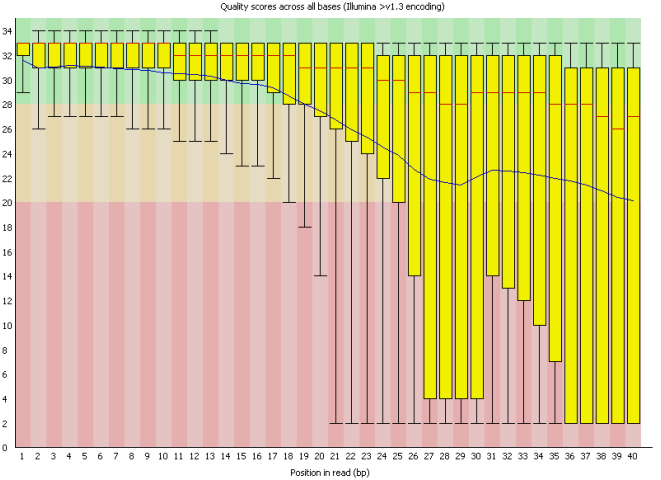
\includegraphics[width=0.5\textwidth]{figures/FastQC_per_base_sequence_quality.png}
  \end{center}
  \label{fig:fastqc_per_seq_qc}
\end{wrapfigure}
\autoref{fig:fastqc_per_seq_qc} shows an example of the per sequence quality graph. This graph essentially provides a quality score per base sequenced. The x axis shows the number of bases, in this case 1 to 40, indicating that at most, 40 bases were sequenced in a row. The y axis represents quality, with the higher score indicating a higher quality. Each instance of the x axis shows a boxplot which represents the quality range (with error margins) of all bases at the number 1 position within the fastq file.\\
If a file is of good quality we expect a majority of early bases to be of high quality (in the green) and the quality would progressively drop as we continue through the x axix, \autoref{fig:fastqc_per_seq_qc} is a good illustration of a good file. However we would hope that the median (red bar in the boxplot) never drops into the lower part of the plot (orange/red color).\\
Things to look out for are abnormal/erratic curves or large `bumps' in the data. Essentially we would expect a relatively smooth curve, if this is not the case we would need to further investigate (using the other elements of this report) to understand if these abnormalities are perhaps an expected biological aspect of the experiment or if something went wrong with the sequencing.\\
The result format seen in \autoref{fig:fastqc_per_seq_qc} also come in a line plot format, in the report this is called `Pre sequence quality scores'.

\subsection{Per base sequence content \label{subsec:fastqc_seq_content}}
\begin{wrapfigure}{r}{0.5\textwidth}
  \begin{center}
    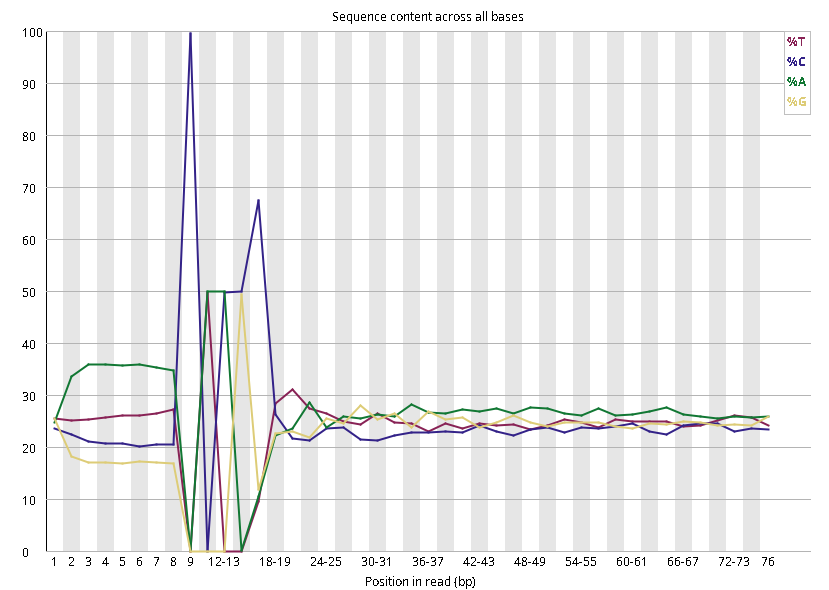
\includegraphics[width=0.5\textwidth]{figures/FastQC_per_base_seq_content.png}
  \end{center}
  \label{fig:fastqc_per_seq_content}
\end{wrapfigure}
As the name indicates this plot shows the distribution of nucleotide type along the x axis of number of bases. Red shows the \%T, blue is \%C, green is \%A, and yellow is \%G. Note that in cases of RNAseq, or other sequencing methods were we include random priming (such as sBLISS) the first n number of bases will likely be erratic, thus throwing an error or warning in the report. For example in \autoref{fig:fastqc_per_seq_content} we see the results of an sBLISS file. The first 8 bases are a bit odd as they represent UMIs, while bases 9-18 are extremely erratic as these are sample barcodes. After this barcode we observe a very normal distribution. Therefore even though FastQC would throw an error for this behaviour, in the context of our experiment it is what we would expect.\\
In the event that strong biases are observed in what would be genomic regions of the file, it is possible that there was a contamination in the library or an error occurred in the sequencing of the library. In either case the error is likely at the lab or sequencing level and not much can be done at the data processing level.

\subsection{Per sequence GC content \label{subsec:fastqc_GC_content}}
\begin{wrapfigure}{r}{0.5\textwidth}
  \begin{center}
    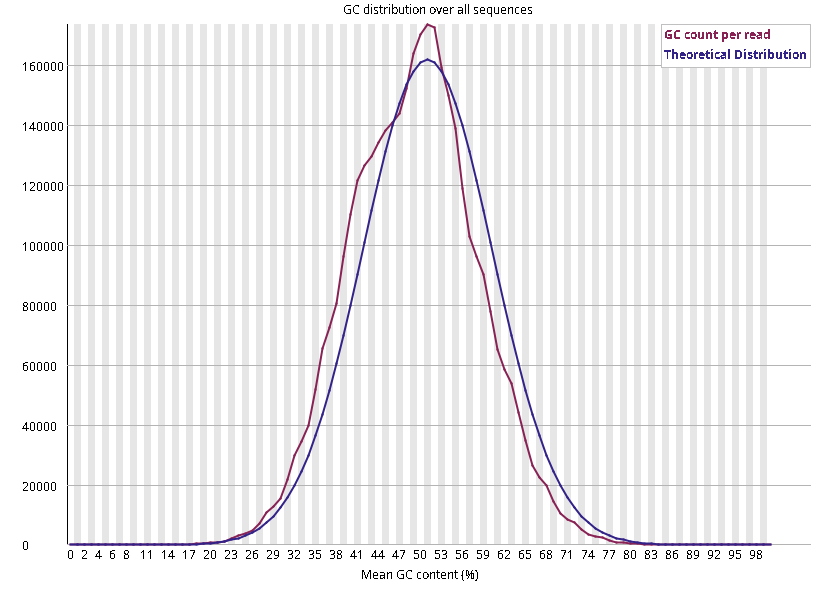
\includegraphics[width=0.5\textwidth]{figures/FastQC_GC_content.png}
  \end{center}
  \label{fig:fastqc_GC_content}
\end{wrapfigure}
For this set of results we expect a normal distribution where the central peak more or less corresponds to the expected GC content for the organism being sequenced. Note that FastQC provides a curve for the theoretical distribution of the GC content (blue curve), however this is calculated based on the data and is not representative of the expected curve for the particular organism. Users can check the work of Romiguier et.al \cite{romiguier2010contrasting} where the expected GC content of 33 different mammals is shown. For convenience, humans are expected at around 46.1\% and mice at 51.24\%. Unfortunately they have not looked at C.elegans, for this we turn towards other studies such as one from John E Sulston and Sydney Brenner \cite{sulston1974dna} which show that the expected GC content for C.elegans is 36\%.\\
In our example dataset taken from an sBLISS protocol we have a human sample whose distribution is slightly shifted \autoref{fig:fastqc_GC_content}. The peak lines up with ~50\% as opposed to 46\%. The cause of this shift may be due to the presence of both UMIs and sample barcodes at the start of each of the sequences, in any case it is not a large shift and would not hinder the continuation of the analysis.\\
If the curve is not a normal distribution or has abnormal bumps it is likely indicative of a contaminated library. This type of issue should be flagged by FastQC. However if the curve is shifted, say in a human sample the peak of the curve lines up with 35\% instead of close to 46\% then FastQC will not flag this as an error although this would be cause for concern. A shift such as this would be reflective of some sort of systemic bias. Another possibility is that the actual curve is far higher than the theoretical curve (same peak location on the x axis but the amplitude on the y-axis is much more significant). In this case it essentially states that the data contains more fragments with GC content than expected. This could be normal or represent a contamination. In the event of a contamination we would expect Fast Screen, a secondary quality control measure, to pick it up.

\subsection{Per base N content \label{subsec:fastqc_N_content}}
In sequencing an `N' is added when the sequencer was incapable of reading a A, T, C, or G. The plots for this section show the percentage of N inclusion at each base position. In an ideal world we see little to no Ns in our data, though it isn't abnormal to see some small bumps here and there, particularly in the higher base numbers (further on the x axis). Though it is subjective, while there are no bumps above the 10\% mark I would consider the data to be okay.

\subsection{Sequence length distribution \label{subsec:fastqc_seq_length}}
\begin{wrapfigure}{r}{0.5\textwidth}
  \begin{center}
    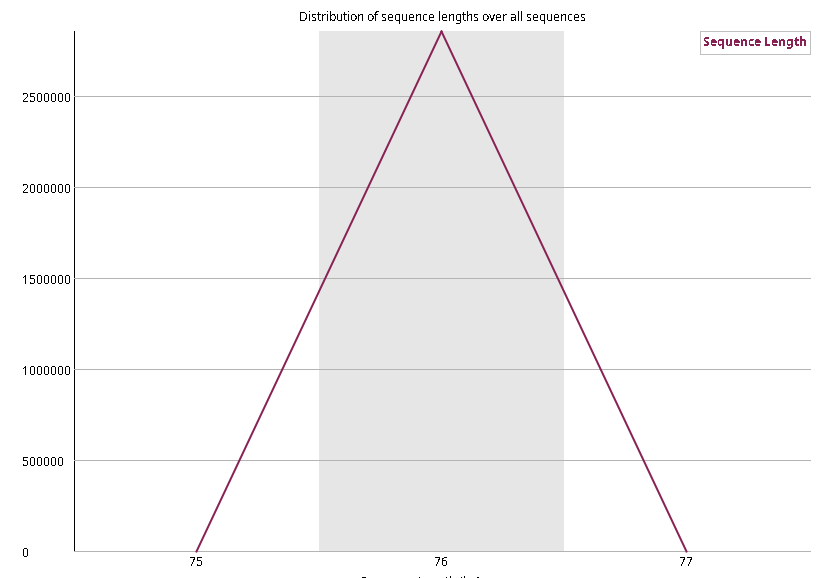
\includegraphics[width=0.5\textwidth]{figures/FastQC_seq_length_distribution.png}
  \end{center}
  \label{fig:fastqc_seq_length}
\end{wrapfigure}
This is another section which is relatively complicated and produces varying results depending on the experiment being done. In addition it isn't the most intuitive set of results. In short, sequencers may generate fragments of uniform lengths or not. The graph of this section shows the distribution of fragment sizes. Generally we expect one large peak, the x axis location of this peak is not incredibly relevant. In our sBLISS examplke dataset seen in \autoref{fig:fastqc_seq_length} we see one large peak at 76bp. This essentially shows that all our reads are 76bp in length. This is a concrete example of a uniform size distribution. This link(\url{https://www.bioinformatics.babraham.ac.uk/projects/fastqc/Help/3\%20Analysis\%20Modules/7\%20Sequence\%20Length\%20Distribution.html}) shows an example of a non-uniform distribution of sizes. The cases where this plot would show cause for concern is if the curve of a non-uniform distribution is erratic, or if the length is much shorter than expected.

\subsection{Sequence Duplication Levels \label{subsec:fastqc_seq_dup}}
\begin{wrapfigure}{r}{0.5\textwidth}
  \begin{center}
    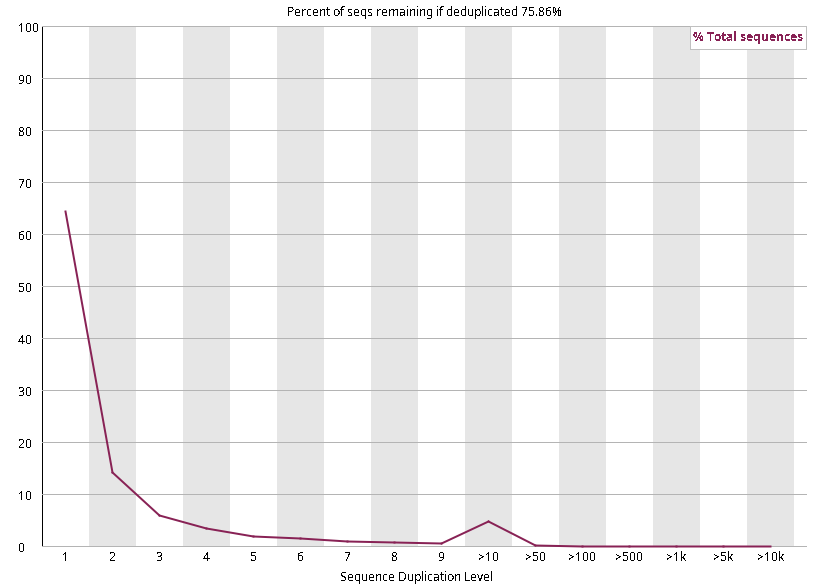
\includegraphics[width=0.5\textwidth]{figures/FastQC_seq_dups.png}
  \end{center}
  \label{fig:fastqc_seq_dups}
\end{wrapfigure}
As the name implies this plot shows the level of duplicated sequences. The y axis is a percentage while the x axis is a duplication level. The plot, fragments (or sequences) which are only observed once are found on the `1' of the x axis. Sequences which are found twice are on the `2' of the x axis and so on. The y axis therefore shows us the percentage of sequences which appear once, twice, and so on until we've checked all sequences.\\
In an ideal world we would expect a large peak at `1' on the x axis and a sharp drop off to then have a plateau at 0. Depending on the type of experiment performed this may not always occur. For example in our sBLISS results \autoref{fig:fastqc_seq_dups} we see the `ideal' scenario however there is a small bump at the 10th level. This indicates that there is a small group of fragments which are very overrepresented. Within the context of our data we assume that this is due to the presence of the sample barcode (adaptors). If these were to be trimmed (removed) this bump would likely disappear.\\
Another possibility is to observe a sharp peak on the later end of the plot, this would indicate that the library used is not very diverse and therefore most fragments have been sequenced multiple times over. This is not inherently an error, but it does show that money may be saved by diversifying, or mixing the library in future iterations of the sequencing.\\
In other instances bump in the curve may appear throughout the plot showing that there are varying levels of duplication. This kind of situation could be either technical or biological in nature. There is no guideline for this kind of event other than attempting to find a biological cause for this behaviour, if one cannot be found it is likely technical in origin. Note that RNAseq often has this kind of profile as in order to observe very scarce fragments, we would inevitably have to over-sequence the prevalent fragments.\\
NOTE: FastQC does not actually check all sequences for this module as this would not be memory efficient from a computing perspective. Instead it creates these results for the first 200 000 sets of sequences. These results are still important, however it is noteworthy to understand that they are not representative of the entire file.

\subsection{Overrepresented sequences \label{subsec:fastqc_overrep}}
This one is a bit more straight-forward. This section will show you if a or several particular sequences/fragments are overrepresented in the file. This could mean that these sequences are of particular importance or it could mean that they are some sort of contamination. All sequences appearing more than 0.1\% of the total are shown. It is likely that if `bumps' are seen in the sequence duplication levels that the cause of these bumps appears in the overrepresented sequences. This may provide the opportunity to identify the cause: contamination, biological significance, or perhaps adapters ect...\\
Note that only the first 200 000 sequences are queried and therefore the results are considered an overview, they do not represent the entirety of the data.


\subsection{Adapter content \label{subsec:fasctqc_Adapter}}
This area simply shows the presence of certain adapter types along the found sequences. This plot can be a helpful tool to customize the trimming component of the pipeline \autoref{sec:trimming}. However in most cases a customized trimming will not be required.

\section{Fast Screen \label{sec:Fast_Screen}}
Fast screen is a much simpler quality control tool when compared to FastQC. In short, Fast Screen attempts to map the found sequences to several genomes. This is meant to serve as a means to evaluate contamination presence and amounts.\\
The results are shown as an HTML file and TXT file, with the HTML file containing a table and plot while the TXT file only contains the table.\\
As an example, \autoref{tab:fast_screen} shows the Fast Screen results for one of the example control files in an sBLISS experiment. Specifically this file contained human data. The important columns are the hits/multi-hits column as these indicate where reads have been mapped. In an ideal world all reads are one hit to one genome, with that genome being the one you sequenced. Having multiple hits on a single genome is to be expected as well. Some possible cases are discussed below.\\
\clearpage
\begin{itemize}
\item Good sample - illustrated in \autoref{tab:fast_screen}.\\
There are mostly hits on a single genome, with some hits on adapters. In this case hits on adapters are expected due to the nature of the sBLISS protocole (see \autoref{sec:sBliss_adaptors}).
\item Contaminated samples\\
In the case of contaminated samples we would likely see several `one genome' results across multiple genomes. This would be a clear sign of contamination.
\item Low complexity reads\\
In this scenario we expect to see mostly multiple-genome results and very few single genome results. This means that the reads obtained are of insufficient quality to be reliably mapped.
\end{itemize}
\begin{table}
\small
\caption{Table showing the results of Fast Screen on one of the example control samples for the sBLISS pipeline} 
\begin{tabular}{|p{.11\textwidth}|p{.05\textwidth}|p{.1\textwidth}|p{.12\textwidth}|p{.12\textwidth}|p{.15\textwidth}|p{.15\textwidth}|}
 \hline
 Genome & Reads & Unmapped & \makecell{One hit/\\one genome} & \makecell{Multi-hits/\\one genome} & \makecell{One hit/\\multi-genomes} & \makecell{Multi-hits/\\multi-genomes}\\
 \hline
 Human & 98403 & 19666 & 53470 & 18418 & 653 & 6196\\
 \hline
 Mouse & 98403 & 93107 & 8 & 5 & 1419 & 3864\\
 \hline
 Rat & 98403 & 92647 & 11 & 6 & 948 & 4791\\
 \hline
 Drosophila & 98403 & 97183 & 1 & 1 & 227 & 991\\
 \hline
 Worm & 98403 & 97872 & 5 & 0 & 274 & 252\\
 \hline
 Yeast & 98403 & 97782 & 0 & 0 & 22 & 599\\
 \hline
 Arabidopsis & 98403 & 97482 & 0 & 0 & 225 & 696\\
 \hline
 Ecoli & 98403 & 98403 & 0 & 0 & 0 & 0\\
 \hline
 rRNA & 98403 & 95075 & 0 & 13 & 79 & 3236\\
 \hline
 MT & 98403 & 98153 & 0 & 0 & 234 & 16\\
 \hline
 PhiX & 98403 & 98403 & 0 & 0 & 0 & 0\\
 \hline
 Lambda & 98403 & 98403 & 0 & 0 & 0 & 0\\
 \hline
 Vectors & 98403 & 98036 & 7 & 0 & 272 & 88\\
 \hline
 Adapters & 98403 & 92235 & 1403 & 4502 & 0 & 263\\
 \hline
\end{tabular}
\label{tab:fast_screen}
\end{table}

\section{MAPQ\label{sec:MAPQ}}
MAPQ stands for MAPping Quality. Unfortunately MAPQ suffers from having multiple methods and definitions depending on the tool used. Samtools sets MAPQ as a range of 0 to 255 with 255 being high confidence mapping. MAPQ is calculated by mappers and some seem to have set ceilings, although this is not explicit in their documentation. Some blog posts have found that bwa has a maximum threshold of 37 while bowtie2 has a maximum of 42 (\url{https://www.acgt.me/blog/2014/12/16/understanding-mapq-scores-in-sam-files-does-37-42}). However bwa has two methods of mapping, one which results in a maximum score of 37 while the other gives a maximum score of 60. This means that for bwa mapped files which used `mem', a q threshold of 60 is essentially selecting for the best confidence possible.\\
This not only illustrates the difficulty in using the MAPQ metric, but also it's inconsistency. This constitutes a relatively large point of debate in the bioinformatic community, that is if MAPQ scores can be trusted/used. There is no widely accepted consensus.\\
This toolbox will use what the pipelines contained within it originally come with, for example sBLISS filters for a MAPQ of 60 when using BWA, meaning the highest confidence of mapping from this tool. GLOE-seq uses a filter of 30 for a bowtie2 aligned file, with bowtie2 having a maximum cap of 42. Based on the way bowtie2 does it's calculation this filter mostly removes reads that are considered to be multi-mapped, that is they can be mapped to more than one location on the genome.\\
In the event where the toolbox is not following a set pipeline no MAPQ filter will be applied. \todo{update with final opinion.}

\section{QualiMap \label{sec:qualimap}}
Qualimap is a tool to perform some quality control metrics on aligned data \cite{qualimap,qualimap2}. This tool differs from previously discussed tools such as Fastqc (\autoref{sec:fastqc}) which perform quality control on as of yet unaligned data. Though the uses of qualimap are diverse this toolbox uses the basic function called bamqc which generates a pdf report on the quality of a single BAM file. There is some overlap between Fastqc and bamqc, with the main similarity being that they both give measure of GC content distribution as well as mapped reads nucleotide content (per base sequence content), for these elements, refer to \autoref{subsec:fastqc_GC_content} and \autoref{subsec:fastqc_seq_content} respectively. Bamqc also covers duplicated reads, similar to \autoref{fig:fastqc_seq_dups}. Below we cover the elements that are unique to bamqc.\\

\subsection{Coverage across reference \label{subsec:bamqc_coverage}}
\begin{wrapfigure}{r}{0.5\textwidth}
  \begin{center}
    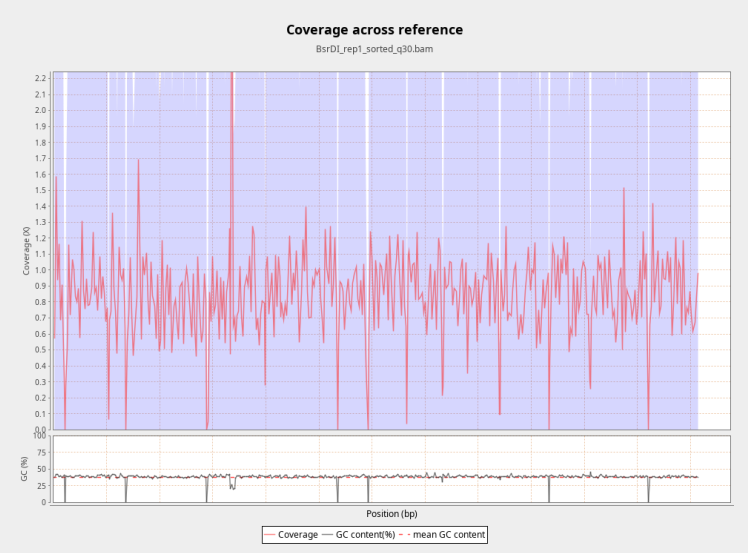
\includegraphics[width=0.5\textwidth]{figures/bamqc_coverage.png}
  \end{center}
  \label{fig:bamqc_coverage}
\end{wrapfigure}
The upper figure shows the coverage distribution while the lower shows the GC content across the reference (black line). The coverage metric (X) equates to the number of reads mapped to each nucleotide of the region, an example can be seen in \autoref{fig:bamqc_coverage}. Put simply, the larger the coverage the more reads in that location of the reference genome. In practice one would expect this graph to relatively inconsistent across the x axis, in other words the coverage is expected to fluctuate quite a bit. In cases where reads are very specific to a location of the genome, one could expect to see a sharp peak at one or few locations as opposed to constant fluctuation. To best utilize this graph one should assess what the protocol has measured and if the expected results correlate with the behaviour seen in this graph. These results are also shown as a histogram which shows the number of reads (y axis) mapped to which coverage (x axis). This histogram also comes with a 50X coverage variant in the event that certain areas of the genome are highly targetted.\\
Similarly there is a plot covering the `Genome Fraction Coverage' which shows the fraction/percentage of the reference associated to a coverage value. It serves as yet another form of visualization for the coverage across the reference.

\subsection{Homopolymer Indels \label{subsec:bamqc_homopolymer}}
\begin{wrapfigure}{r}{0.5\textwidth}
  \begin{center}
    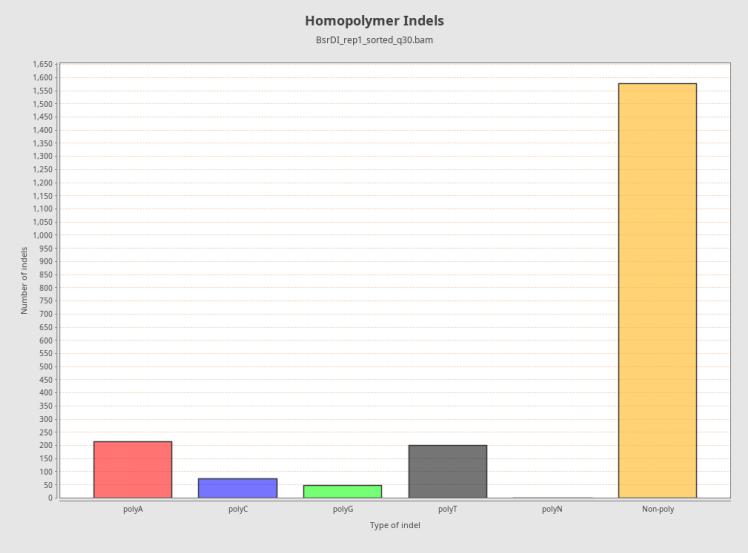
\includegraphics[width=0.5\textwidth]{figures/bamqc_homopolymer.png}
  \end{center}
  \label{fig:bamqc_homopolymer}
\end{wrapfigure}
If indels are present in the dataset, this plot (\autoref{fig:bamqc_homopolymer}) is generated. The official definition of this plot is "this plot shows separately the number of indels that are within a homopolymer of A’s, C’s, G’s or T’s together with the number of indels that are not within a homopolymer". In the context of DNA, a homopolymer is a series of identical nucleotides, perhaps the most common example being a polyA tail. BamQC defines a homopolymer as being at least 5 consecutive identical nucleotides. Homopolymers are known to cause difficulties in sequencing in addition to having increased error rates when compared to other areas of the genome \cite{kunkel2004dna,fazekas2010improving}. This metric on it's own cannot say if a mapping is good or bad, but it can serve as an indication of the certainty of mapping for areas which are rich in homopolymers. This can be taken into account when interpreting results. In the event that the amount of indels are overwhelmingly high it may indicate an issue with the sequencing itself. In the example figure given the statistic if roughly 25\% of reads are indels (this value is found in a table of the report but not in the plot). This would be a case where the amounts would be considered `overwhelmingly high'. In this case, the dataset originates from an example fastq file which is not expected to produce meaningful results.

\subsection{Mapping Quality Histogram \label{subsec:bamqc_mapq}}
\begin{wrapfigure}{r}{0.5\textwidth}
  \begin{center}
    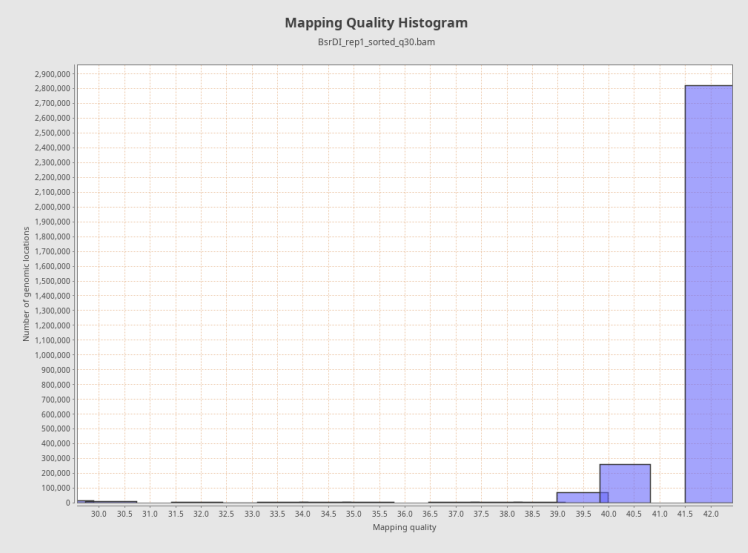
\includegraphics[width=0.5\textwidth]{figures/bamqc_mapq.png}
  \end{center}
  \label{fig:bamqc_mapq}
\end{wrapfigure}
This plot gives a visual representation of the quality of mapping (MAPQ). More information about this metric can be found in \autoref{sec:MAPQ}. This graph is quite useful in determining if the file could benefit from a MAPQ based filter. In the case of \autoref{fig:bamqc_mapq} the results shows scores only above the 30 score as this BAMQC was performed on a bam file which has already been submitted to a MAPQ filter of 30.

\fancyhead[RO]{Tools}
\mychapter{7}{Tools}
\label{chap:tools}

\section{Trimming \label{sec:trimming}}
As the name implies, trimming is the act of trimming down reads. It's most basic application is to remove left over adapters from the reads, as in some cases these adapters can interfere with the mapping process \autoref{sec:mapping}. Similar to other steps of data processing, several tools exist to trim fastq files, some of the more common ones are listed below:\\
\begin{itemize}
\item Trimmomatic \cite{bolger2014trimmomatic}
\item CutAdapt \cite{martin2011cutadapt}
\item Trim galore \cite{krueger2015trim} - This is a wrapper of FastQC \autoref{sec:fastqc} and cutadapt, which means that it utilizes FastQC to find the quality of reads as well as the adaptors, it then uses cutadapt to trim these per the users requirements.
\end{itemize}
Trimming is often used to remove adaptors, however it is also used for `quality trimming' that is the removal of low-quality reads if they are present. This is one of the reasons why fastq files contain the read sequenced along with the quality score of that read \autoref{sec:Fastq_files}. By giving a tool a threshold of quality it can remove any reads which fall below that quality threshold. Another facet of quality trimming is the removal of reads which are too short once adaptors have been removed, though the use of this step is often very dependant on the experiment performed. For example in RNAseq we would expect to do this every time otherwise the reads would be too difficult to map accurately. In cases such as 
sBLISS trimming is also performed, however this is done for both UMIs and adaptors. Since UMIs are by definition unique, the default parameters of a trimmer would not remove these. The tools within this toolbox account for this, this statement simply illustrates the thought process sometimes required to use a trimming tool.\\
For pipelines which do not come equipped with a preferred trimmer, this toolbox will favour the use of Trimmomatic due to having prior experience with the tool. For convenience, the Trimmomatic set-up in the pipelines will simply look for all known adapters, this decision was made to limit the amount of parameters a user would have to input, in this case a user does not need to know the specific adapters used for their data. Looking for all adaptors should not impact the data in any negative way as all adapters are designed to not be `seen' as known DNA sequences.

\section{Mapping \label{sec:mapping}}
Mapping is the process of determining the location of a read on the genome, thus associating reads to specific genomic elements, and eventually specific genes. In bioinformatics we have several tools for this, some of the more commonly used ones are listed below:
\begin{itemize}
\item Burrows-Wheeler Aligner, BWA for short \cite{bwa1,bwa2}
\item Bowtie2, which also utilizes the Burrows-Wheeler approach \cite{bowtie2}
\item HISAT2 (hierarchical indexing for spliced alignment of transcripts), which is more commonly used to generate RNAseq count data \cite{hisat}
\item START (Spliced Transcripts Alignment to a Reference) is another commonly used aligner for RNAseq count data \cite{star}
\end{itemize}
The above listed are but a selection of the aligners available. As can be seen aligners usually have a specialization, where BWA and Bowtie are most often used for data where genomic location, in addition to exons, are of interest. While other aligners designed for RNAseq in mind, focus on spliced (exonic) transcript alignment. There is much debate in regards to which alignment is best, and ultimately the best aligner will depend on the experimental need.\\
This toolbox will prioritize the use of the aligner specified by a pipeline. For example the authors of the sBLISS protocol use BWA, therefore this toolbox also utilizes BWA for that protocol. However for standard Chip-seq and ATAC-seq the toolbox uses Bowtie2 due to it's familiarity.\\
For the RNAseq pipeline STAR is used, again this is simply due to the author's familiarity with it.\\
Musich et. al. wrote a small review comparing some of the aligners above from the point of view of a biologist \cite{musich2021comparison}, it may be an interesting read to some.

\subsection{Genome reference files}
Genome reference files are usually found as `.fa' files. These are usually downloaded from a GRC (Genome Reference Consortium). For example the most up to date murine and human genomes can be found at Gencode (\url{https://www.gencodegenes.org/}). These files are relatively large and it would be computationally demanding to utilize them as they are, for this purpose modern mappers require that the downloaded `.fa' files be indexed before mapping. This often involves a simple command line execution, however users of this guide need not worry about it unless their desired reference genome is not include. For a list of included reference genomes see \autoref{subsec:included_genomes}.\\
The purpose of indexing is that it splits up the reference file and allows the tool to only load segments at a time instead of the entire file. Note that each tool has their own version of indexing. They are relatively similar however they do require that indexing be performed using their tool. For example, the indexes generated by bowtie2 will not be compatible with BWA. Since Bowie2, BWA, and STAR are aligners used within this pipeline, below are the three methods of generating gene indexes for each aligner respectively.

\begin{itemize}
\item Bowtie2
\begin{lstlisting}
bowtie2-build path/to/reference.fa --name pick_name
\end{lstlisting}
\item BWA
\begin{lstlisting}
bwa index path/to/reference.fa
\end{lstlisting}
\item STAR
\begin{lstlisting}
STAR --runThreadN 6 \
--runMode genomeGenerate \
--genomeDir target_directory \
--genomeFastaFiles path/to/reference.fa \
--sjdbGTFfile path/to/gene_annotation.gtf \
--sjdbOverhang 99
\end{lstlisting}


\end{itemize}

\subsection{Included genomes \label{subsec:included_genomes}}
This toolbox includes many reference genomes:\\
\begin{itemize}
\item GRCh38 - Human
\item GRCm38 - Mouse
\item WBcel235 - Celegans
\item R64-1-1 - Saccharomyces cerevisiae (Yeast)
\item Rnor\_6.0 - Rat
\item TAIR10 - Arabidopsis Thaliana
\item BDGP6 - Drosophila melanogaster
\item Ecoli
\end{itemize}
Note that additional genomes can be added upon request.\\
\todo{T2T?}
\subsection{Blacklisted regions \label{subsec:blacklisted_regions}}
An important element to Chip-seq and other associated technologies is to account for blacklisted regions. For this we specifically refer to the work carried out by ENCODE \cite{amemiya2019encode}. They define their blacklisted regions as "a comprehensive set of regions which have anomalous, unstructured, or high signal in next-generation sequencing experiments independent of cell line or experiment". They claim that the removal of these regions is an essential quality control measure. Genomes with blacklisted regions are the following:\\
\begin{itemize}
\item HUMAN (hg38)
\item HUMAN (hg19)
\item MOUSE (mm10)
\item MOUSE (mm9)
\item WORM (ce11)
\item WORM (ce10)
\item FLY (dm6)
\item FLY (dm3)
\end{itemize}
All of these files are contained in the toolbox. They can also be downloaded here (\url{https://github.com/Boyle-Lab/Blacklist/tree/master}).\\
Since these blacklists do not exist for all genomes users would have to be aware of this absence of quality control if they utilize a genome for which a blacklist is not available. Importantly this is only required for Chip-seq and Chip-seq derived methods. RNAseq would be exempt from this filtering as the blacklisted regions do not correspond to exonic areas of the genome, therefore the captured mRNA would not map to blacklisted locations. The authors also showed that blacklisting is not productive for WGS.\\
Importantly, the elements of this toolbox handles the removal of blacklisted elements in the analysis sections of the pipelines. This choice was made to clearly show the users that this step is occurring and it makes it easier to exclude this filtering step. This may be required if one is studying protein coding genes in unmappable regions of the genome as these regions would removed by the blacklist.

\section{Sorting with Samtools \label{sec:samtools}}
Samtools is a toolbox of it's own, one that is used to interact with high-throughput sequencing data \cite{li2009sequence}. One of the main functions of Samtools is called `sort', which as the name describes it allows us to sort the aligned BAM files in different ways. Another important function, and the one we focus on in this text, is `view'. The primary use of `view' is to convert a SAM file into a BAM file (see \autoref{chap:File_types}) however it also allows us to select for a quality metric called MAPQ \autoref{sec:MAPQ}. It is common for tools to select for aligned reads above a certain quality metric. In this toolbox if a quality metric has been selected the resulting file (a bam file) will carry a name indicating the threshold that was used, for example `test\_file\_q\_60.bam' which would indicate that a value of 60 was used for the filter. To better understand what these values represent see \autoref{sec:MAPQ}. By default some tools of this toolbox may use the quality threshold version, however a non-quality filtered bam file is also produced in the event that a user may prefer that output.

\section{Peak Calling \label{sec:peak_call}}
Peak Calling is a means to identify areas of the genome which have been enriched in aligned reads. The main tool used for peak calling is MACS, which now has three variations MACS1 to 3. This toolbox uses the MACS3 \cite{MACS3}.\\
MACS stands for `Model-based Analysis for ChiP-Seq'. It was initially developed for the analysis of ChiP-Seq data however it can be used in ChiP-Seq derived protocols, however it's use may be different depending on the variant. For example, MACS offers a very convenient comparison function where a `treatment' along with a control can be provided, from this it can identify peaks relevant to the `treatment' provided. However in the case of sBLISS, which contains many more hits along the genome than a traditional Chip-Seq analysis, the control-treatment comparison often fails. In these cases it is best to simply run MACS on the treatment sample and do the comparison with the control during the data analysis step.\\
When MACS is used without a control, what it identifies changes. One could say that it identifies statistically significant peaks. The wording they use is: \textit{finding significant reads coverage than (compared to) the random background.}\\
MACS is a relatively diverse tool which allows for a variety of functions however in this tool box we focus on the `callpeak' function. The tutorial and documentation can be found here (\url{https://macs3-project.github.io/MACS/docs/Advanced_Step-by-step_Peak_Calling.html}) and here (\url{https://macs3-project.github.io/MACS/docs/callpeak.html}) respectively.\\
The input file for peak calling is often a .bam file with it's associated .bai file (see \autoref{sec:BAM_files}) however it can utilize other file types. Within the context of this toolbox all uses will be done using .bam files. This represents a fastq file that has been mapped.\\
MACS3 produces a variety of results, but the one that is particularly interesting is the `narrowPeak' output. The column names can be seen in \autoref{fig:MACS3_output}. 
\begin{figure}
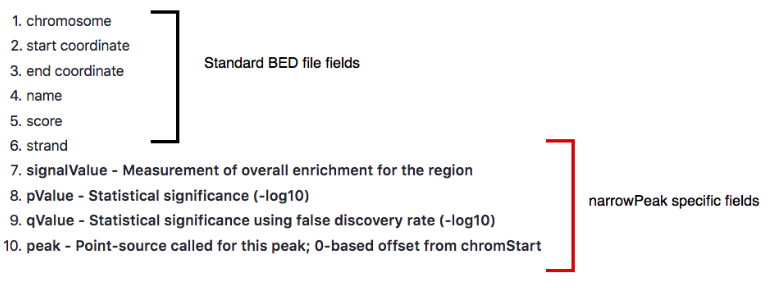
\includegraphics[width=\textwidth]{figures/MACS3_peakcall_output.png}
\caption{The output format for peak (narrow) calling using MACS3. It is found as a `.bed.narrowPeak' file extension.}
\label{fig:MACS3_output}
\end{figure}
For those interested there is a detailed guide on peak calling found here (\url{https://hbctraining.github.io/Intro-to-ChIPseq/lessons/05_peak_calling_macs.html}. It covers some important parameters and details on how peak calling works. One of these is highlighted below due to it's importance in experimental design and impact on biological interpretation.

\subsection{Understanding duplicates \label{subsec:MACS3_dups}}
In MACS3 there is a parameter called -{}-keep-dup which allows the user to keep or remove duplicates. This brings up a relevant biological question as to what is a duplicate in the context of peak calling and why these may be good or bad. For MACS a duplicate is a read which appears in the same location (in both strand and chromosomal coordinates). By default it preserves one instance per strand, though all duplicates can be preserved if desired. To better understand this we first need to understand what are good and bad duplicates. In brief: \\
\begin{itemize}
\item Good duplicates: In some biological cases one could expect many hits in similar or identical coordinates. This is particularly true in Chip-seq if the targetted protein only binds to a few sites. In this case, if you have a good amount of biological replicates, preserving duplicates is important as if they are not kept it may lead to an under-representation of the results.
\item Bad duplicates: Biases in PCR may lead to bad duplications, or in other words, artificially enriched regions, this may occur if the initial starting material (pre-PCR) is low. One may also need to be wary of blacklisted regions, that is regions which are known to produce large amounts of duplicates. To handle both of these issues one can remove duplicates. 
\end{itemize}
In the event where only blacklisted regions are a concern these can be filtered out in some steps of the pipeline. I prefer to filter them in the analysis step of the pipeline, similar to what is seen in the SBLISS PIPELINE STEP OF BLACKLIST \todo{don't forget this ref}.\\
Another method of avoiding bad duplicates is to leverage UMIs. In some protocols such as sBLISS \autoref{chap:BLISS_sBLISS} there are UMIs, where a duplicated UMI would represent a bad duplicate, while if the UMIs are different, but their location is the same, they would be good duplicates.\\
\textbf{In general, best practice is to follow the default behaviour of the pipeline, which is to remove duplicates.}


\section{Counting features \label{sec:featureCounts}}
In the case of RNA sequencing we `count' the number of reads aligned to any given gene. To do this we utilise featureCounts \cite{liao2014featurecounts}. At it's most basic featureCounts takes in a BAM file, in our case the file would be from the STAR aligner. The tool also requires an annotation file (or gtf file). The annotation file contains the name of genes, their characterization (exon, intron, ect...) as well as it's chromosomal location. In standards bulk RNAseq featureCounts will extract all exonic gene ids and match their location in the BAM file. By then counting the number of reads in that location it would obtain the number of counts for a given gene.\\
One issue that can arise between STAR and featureCounts is that the chromosome names can vary from the reference genome to the annotation file, this is largely dependant on how the reference genome was built. In our pipeline when building the STAR reference genome for GRCh38, the chromosome names ended up being swapped with GRCh38, for example chr\_1 and chr\_y became GRCh38\_1 and GRCh38\_y. Hence we adjusted the annotation file to have the same naming format. This error can be seen after an initial run of the pipeline where the `count summaries' (produced by featureCounts upon completion) states that there are many unassigned reads and 0 assigned reads, meaning none of the reads found could be matched to a location in the annotation file. If this error is observed, check the reference genomes nomenclature and verify that it matches the annotation file's nomenclature.

\fancyhead[RO]{File Types}
\mychapter{8}{File types} 
\label{chap:File_types}
Several file types exist. Note that many of these are massive files that should not be opened (double clicked). If you are curious about their content, which may be usefull for checking the format, you can use a tool such as Glogg which allows you to visualize large text based files \autoref{sec:glogg}.

\section{Fastq files \label{sec:Fastq_files}}
At it's core Fastq files are a text based format to store biological sequenced. This format was created to merge FASTA files and their associated quality metrics into a single file. Note that FASTA (or .fa) formats are also text based files but they are meant to only contain an identifier and a sequence. Looking at the example below, a FASTA format would not contain the information found between the colons on the first line.
\begin{formal}
\hlgreen{@HWI-ST1276:71:C1162ACXX:1:1101:1208:2458 1:N:0:CGATGT}\\ 
\hlorange{NAAGAACACGTTCGGTCACCTCAGCACACTTGTGAATGTCATGGGATCCAT}\\
+\\
\hlblue{\#55???BBBBB?BA@DEEFFCFFHHFFCFFHHHHHHHFAE0ECFFD/AEHH}
\end{formal}
The example above is from a random NOVOGENE sequenced file. In green we see the header with the @ preceding the identifier, this is followed by information concerning the machine: HWI-ST1276 is the unique identifier of the sequencer used. 71 refers to the run number on the instrument. C1162ACXX is the identifier for the flow cell, 1 is the lane number, 1101 is the tile number. The x and y coordinates of the tile are 1208 and 2458 respectively. The 1 is the number of reads, this can also be 2 in the event of paired-end sequencing. N (or Y) stands for Yes/No depending on if the read passed filtering or not (QC). 0 shows the number of control bits. Finally CGATGT is the illumina index sequences. In some instances we also have a length of read given after the header.\\
The sequenced read is shown in orange\\
Following the `+'  indicating that the information that follows is associated to the previously observed header. Some machines/protocols have the same header appended after the `+'. What follows the `+' is the quality values (in blue). These quality values are not meant to be readable by humans.\\
As previously stated, not all fastq files are formatted the same way, due to this it is important to understand the general layout of the files, but also know which machine produced the files and search exactly what that machine has produced.

\section{BAM and SAM files \label{sec:BAM_files}}
BAM stands for Binary Alignment Map, generally we obtain BAM files once a fastq file has been mapped (see \autoref{sec:mapping}). BAM is the condensed version of a SAM file (Sequence Alignment Map), with this in mind it makes more sense that BAM relates to mapped files. In computer science a condensed version essentially translates to a more light-weight (in terms of bytes) file.\\
A BAM file is (or should be) accompanied by a indexing file. Having an indexing file allows the computer to quickly find specific locations in the file. In essence when looking for something it immediately narrows down the search area in the file as opposed to having to look through the entire file every time. The indexing can be identified as having the same name as the bam file, but followed by a `.bai'\\
Note that BAM files are often large files and therefore should not be opened manually opened (double-clicked). In addition it is a compressed file so the text inside will not be understood by humans.

\fancyhead[RO]{Miscellaneous}
\mychapter{8}{Miscellaneous}
\label{chap:misc}
\section{Single-end vs Paired-end \label{sec:SE_vs_PE}}
\begin{wrapfigure}{r}{0.5\textwidth}
  \begin{center}
    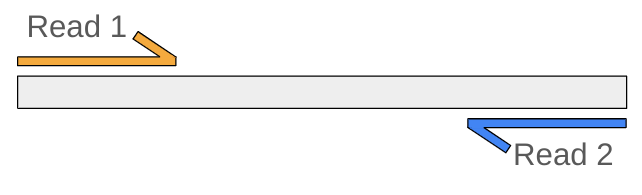
\includegraphics[width=0.5\textwidth]{figures/PE_SE.png}
  \end{center}
  \label{fig:PE_SE}
\end{wrapfigure}
In all pipelines of this toolbox the method of processing of single-end and paired-end sequencing is handle automatically \todo{Are they all adapted?}. However it remains important to understand the difference between these two types of sequencing. The simplest explanation is that single-end (SE) reads/sequences a fragment from a single-end while paired-end (PE) will sequence from both ends. If looking at \autoref{fig:PE_SE} SE would result in only `Read 1' for all fragments while PE would results in both read for each fragment. PE effectively produces twice the amount of reads.\\
The advantage of PE over SE is that PE offers higher quality reads. When sequencing it is expected that the quality of a sequenced read degrades for every base of the fragment (see \autoref{subsec:fastqc_seq_quality}), thus by sequencing from both ends of the fragment we avoid having one end of the fragment being of poor quality. This is particularly useful when we expect fragments to be relatively large, for example in long read RNAseq or in whole genome sequencing. The caveat of PE is that it costs more and requires more computing resources. SE is sufficient for sequencing protocols which generate small fragments such as small RNA-seq as well as sBLISS or Chip-seq.

\section{Glogg \label{sec:glogg}}
Glogg is an application created to browse and search through long or complex files \cite{Glogg}. It was initially designed to look through log files to help programmers find specific locations within a log file, however it can also be used to visualize large genomic files. The search functionality of Glogg is relatively useless for genomic perspectives however visualizing the files allows us to look at it's basic formatting. This is particularly relevant when obtaining Fastq files and checking if it's formatting is compatible with certain tools such as sBLISS \autoref{chap:BLISS_sBLISS}.

\section{Computer terminal \label{sec:terminal}}
The terminal of the computer can be defined in many ways, perhaps the simplest is that the terminal is a direct line of communication from you (the user) to the computer. We consider this a `direct line' as you do not go through a GUI (Graphical User Interface). GUIs are windows which you can scroll, click, and so on. For example, when you want to go to a specific folder and open a file inside it, you will have a window where you can double-click folders and eventually double-click a file to open it. This navigation window is a GUI. That said, the first thing that needs to be known about the terminal is how to navigate through folders.\\
\begin{itemize}
\item Getting a list of files (ls)\\
If you type `ls' in the terminal you will obtain a list of files in your current location.
\begin{lstlisting}
cd seq_toolbox/sbliss/
\end{lstlisting}
\item Changing directories (cd)\\
To change a directory you start by typing `cd' followed by a space and then the name of the directory that you wish to navigate to. The terminal is helpful in the sense that it will assist you with the spelling of your directories/folders. If you hit the `tab' key the terminal will auto-complete as much as possible, if it does not complete the text fully it means that there is more than one possibility. In this case you can hit `tab' twice and it will show you a list of options from the current text. You must then add to the spelling until the remainder of the spelling is unique, at which point you can hit `tab' again and it will autocomplete.\\
The auto-completion when switching looking at folders will only continue to the end of a folder name, the end of a folder/directory is marked by a `/'. At which point you would repeat the previous (type out part of the next folder/file in the sequence and hit `tab').\\
As an example, below I could write out `seq\_' and hit tab, and provided that no other files/folders in my current location start with that name it will complete the entry with `toolbox/', I can then write `sb' and hit `tab' again for it complete the entry with `liss'.\\
Once you have reached your desired location, hit `enter', this will execute the command you have written. In this case your directory will change.
\begin{lstlisting}
cd seq_toolbox/sbliss/
\end{lstlisting}
The above can also be achieved in two separate commands, as seen below.
\begin{lstlisting}
cd seq_toolbox/
cd sbliss/
\end{lstlisting}


\item Navigating backwards or resetting\\
In some instances you may want to go backwards in the directory. One option is to simply write `cd' and hit enter. This will return you to the home directory. An alternative is to write `cd ..' which will go backwards in the directory by one folder. If you were in `A\_projects/seq-toolbox', using `cd ..' will put you in the A\_projects directory.

\item Concatenating files\\
Sometimes a sequencing facility can give fastq files which are separated by lanes. Essentially if the data of one sample is spread on multiple lanes of the sequencer you may obtain as many files as lanes used for that sample. In these instances the files need to be concatenated together. Fortunately there is an easy command to accomplish this, it is appropriately named `cat'. Let's assume we have two files named PFC1\_L3\_1.fq.gz and PFC1\_L3\_2.fq.gz. In this example we know that these two files should be merged together.
\begin{lstlisting}
cd <the directory where the files are located>
cat PFC1_L3_1.fq.gz PFC1_L3_2.fq.gz  > PFC1_L3.fastq.gz
\end{lstlisting}
In the above command we first change the directory to where our files are located. We then call the `cat' command followed by the files we seek to merge, note that this is not limited to two files, one must only ensure that each different file is followed by a space. We then use `>' to indicate the output name, here we will name the product of our merge as `PFC1\_L3.fast.gz'. Upon completion, this new file will be located in the same location as the original files. Note that this does not delete the original files therefore you need to make sure that there is sufficient space/memory on your computer/hard-drive to allow for the creation of this new file.
\end{itemize}

\subsection{Dangers of the terminal}
When using the terminal there are a few things to keep in mind. The most important of which is that a file deleted via the terminal is not recoverable. Files deleted this way are not sent to the trash, they are simply removed. The command to do this is `rm'. For the purpose of this toolbox `rm' will never be required, for this reason I would recommend that those who are unsure of what they are doing DO NOT use the `rm' command. If used incorrectly it is possible to delete key components of a computer's software, thus requiring a full reset of a computer and causing the loss of all data on it.\\
For the curious, if one were to open a terminal, type `rm *' it would delete everything in the current directory. Since the directory in which you open the terminal is the `home' directory, everything save some background folders will be deleted.

\subsection{File permissions}
It is relatively common to encounter errors relating to file permissions, or specifically `permission denied' errors. This translates to a specific file or script not being allowed to read or write in a certain location. This is often due to a file not being considered an `executable', that is a file/process that is supposed to be able to perform an action of some sort, implicitly meaning that it must be able to do changes. To give a file/script the `executable' status we can use a command called chmod which is a shortened version of `change mode'. By using the `+x' parameter we can give a file the `executable' status. Let's say we have a script called `my\_pipeline.sh' which is being denied permission to read/write. We can use the command below to give it the required status/permission. Below we give the +r(read), +w(write) and +x(execute) permissions.
\begin{lstlisting}
cd <the directory where the files are located>
chmod +rwx my_pipeline.sh
\end{lstlisting}


\clearpage
\bibliographystyle{unsrt}
\bibliography{references}


\end{document}
